% glyphlens paper — working draft for co-authors.
%
% Build:  latexmk -pdf main.tex      (or: pdflatex, bibtex, pdflatex, pdflatex)
%
% Conventions (see README.md):
%   \doubt{...}  a claim, reading or citation use that is NOT fully verified;
%                each one says what would settle it.
%   \todo{...}   work the authors still have to do.
%   \annotatefalse (below) hides both, for a clean read — never for submission
%   while any remain.
%
% The class is plain `article` on purpose: the venue is undecided (see
% docs/positioning.md §7). Porting to the IEEE VIS (vgtc) or EuroVis (egpubl)
% template is mechanical once it is.

\documentclass[10pt,twocolumn]{article}

\usepackage[T1]{fontenc}
\usepackage[utf8]{inputenc}
\usepackage{lmodern}
\usepackage{microtype}
\usepackage[margin=0.8in,columnsep=0.28in]{geometry}
\usepackage{amsmath,amssymb}
\usepackage{graphicx}
\usepackage{booktabs}
\usepackage{longtable}
\usepackage{tabularx}
\usepackage{multirow}
\usepackage{array}
\usepackage{enumitem}
\usepackage[dvipsnames]{xcolor}
\usepackage{tikz}
\usetikzlibrary{arrows.meta,positioning,decorations.pathreplacing,calc}
\usepackage{pgfplots}
\pgfplotsset{compat=1.18}
\usepgfplotslibrary{fillbetween}
\usepackage{subcaption}
\usepackage[numbers,sort&compress]{natbib}
\usepackage[hidelinks]{hyperref}
\usepackage{doi}
\usepackage{cleveref}

% --- annotations -----------------------------------------------------------
\newif\ifannotate
\annotatetrue
\ifannotate
  \newcommand{\doubt}[1]{{\color{BurntOrange}\,[\textbf{?}\,#1]}}
  \newcommand{\todo}[1]{{\color{BrickRed}\,[\textbf{TODO}\,#1]}}
\else
  \newcommand{\doubt}[1]{}
  \newcommand{\todo}[1]{}
\fi

% Audit table: author, year and number of a source.
\newcommand{\src}[1]{\citeauthor{#1}~\citeyear{#1}~\cite{#1}}

% --- names -----------------------------------------------------------------
% One place to change the system's name: "GlyphLens" is already the title of
% Tong, Li & Shen (TVCG 2017), so the library needs renaming before submission.
\newcommand{\sys}{\textsf{glyphlens}}
% Pipeline stages. Tominski et al.'s model uses sigma, lambda and bowtie.
\newcommand{\Sel}{\sigma}
\newcommand{\Bin}{\beta}
\newcommand{\Nrm}{\nu}
\newcommand{\Plc}{\varphi}
\newcommand{\Anc}{\gamma}
\newcommand{\Mrk}{\mu}
\newcommand{\Asc}{\rho}
\newcommand{\Jn}{\bowtie}

\title{Bearing-Faithful Map Lenses for Categorical Counts:\\
From a Single Lens to a Gridded Glyphmap%
\todo{working title}}
% Narrowed on 2026-09-25 to what the demonstrations show: one categorical
% variable summarised by count. Widen it only together with a multivariate case
% (see "How multivariate is this?" in the discussion).


\author{Dany Laksono \and Aidan Slingsby \and Radu Jianu%
\todo{affiliations, order and author list to be agreed}}

\date{Working draft --- \today}

\raggedbottom
\begin{document}
\maketitle

\begin{abstract}
A map lens that \emph{summarises} the data under it---rather than magnifying or
filtering it---must decide what to summarise and where to put the summary.
Existing lens models leave both inside a single lens function and join. We
refine them into seven stages (selection, binning, normalisation, placement,
anchor, marks, association) and show that a category ring, a bearing-faithful
necklace, a route profile and a gridded glyphmap are points in one space,
reached by changing arguments. The part of the space we find new is where the
lens boundary itself carries data: aggregates placed on a ring at the bearing of
what they summarise, displaced minimally rather than dropped; a leader that
appears exactly where placement or unrolling has given adjacency away; a ring
that unrolls into an axis without re-solving; within-unit structure read from
the lens's own polar frame; and a radius control that shows how fragile the
reading is. Every demonstration summarises one categorical variable by count:
four classes of OpenStreetMap places in Yogyakarta, as 1{,}449 points and as
counts for 14 districts. We relate the model to lens design spaces, focus-region labelling,
necklace maps and geographically weighted statistics, state which parts we
concede to them, describe an open-source implementation, and set out the
controlled study that the central design claim still requires.
\todo{Rewrite once the study has run; keep to the venue's word limit.}
\end{abstract}

% ---------------------------------------------------------------------------
\section{Introduction}
\label{sec:intro}

Interactive lenses are one of visualization's most general interaction
primitives: a movable region under which the base visualization is shown
differently~\cite{bier1993toolglass,tominski2014star,tominski2017survey}. On
maps, many lenses \emph{magnify}, \emph{filter} or \emph{re-render} what lies
beneath them. Others instead \emph{summarise} it: a probe pairs a
region with charts of its contents~\cite{butkiewicz2008probes}, a time lens
wraps a query circle in a ring of temporal aggregates~\cite{tominski2012stacking},
and a shipped map-lens product draws a bar chart of the data under each lens
around its rim~\cite{visquill}.

A summarising lens has to answer two questions that a magnifier does not. What
is summarised---which members, decomposed how, normalised against what? And
where does the summary go---in which order around the lens, on what curve, and
how is each mark tied back to the ground it describes? In the rings we have
seen, the second question is answered by habit: marks are laid out in category
(or time) order, so the most valuable channel on a ring---angular
position---carries a category or time order and nothing geographic. A bar at eleven
o'clock says nothing about the north-west.

This paper makes three moves. First, we refine Tominski et al.'s lens model
(selection $\Sel$, lens function $\lambda$, join
$\Jn$~\cite{tominski2017survey}) for summarising lenses into seven stages,
$\lambda=\Mrk\circ\Nrm\circ\Bin$ and $\Jn=\Asc\circ\Anc\circ\Plc$
(\cref{sec:model}), and use it to describe existing techniques
(\cref{sec:descriptive}) and to generate new ones (\cref{sec:generative}).
Second, we make angle mean \emph{bearing}: each aggregate is placed on the lens
boundary at the bearing of what it summarises, using necklace-map
placement~\cite{speckmann2010necklace} with minimal displacement; a leader is
drawn exactly where the gap between a mark and its data would mislead; and
because placement is solved in the curve's parameter, the ring unrolls into an
axis without re-solving. Third, we treat the number of lenses as a parameter,
so that one lens, a handful of small multiples and a gridded glyphmap are the
same object, and we are explicit about how much of that continuum is
geographically weighted statistics under another name (\cref{sec:discussion}).

\paragraph{Contributions.}
\begin{itemize}[leftmargin=*, itemsep=1pt]
  \item A seven-stage model of summarising lenses that refines the
    selection--function--join model, with two values the existing lens design
    spaces lack: an effect scope \emph{on the boundary}, and thematic marks
    under a spatial layout (\cref{sec:model}).
  \item Bearing-faithful placement of aggregates on a lens boundary, with a
    residual leader and curvature as a free axis (\cref{sec:placement,sec:association}).
  \item Within-unit structure read from the lens's polar frame, and the
    elasticity of the count with respect to the radius drawn on the radius
    control, positioned against the local point-pattern statistics it
    re-expresses (\cref{sec:within,sec:elasticity}).
  \item The lens-to-glyphmap continuum as one object (\cref{sec:continuum}).
  \item An open-source implementation (\cref{sec:implementation}) and the
    design of the controlled study the central claim requires
    (\cref{sec:evaluation}).
\end{itemize}

\todo{Teaser figure: category ring $\to$ necklace $\to$ unrolled with leaders
$\to$ field, from \texttt{figures/}.}

% ---------------------------------------------------------------------------
\section{Related work}
\label{sec:related}

The closest precedents to a bearing-faithful summarising lens are mostly not
called lenses. They sit in five literatures: interactive lenses and their design
spaces; labelling around a focus region; off-screen indicators on the viewport
border; radial and necklace cartography; and glyph maps with their underlying
local statistics.

\subsection{Interactive lenses and their design spaces}

%%RELATED-LENSES%%

\subsection{Marks around a focus region}

\emph{Excentric labelling} shows the labels of objects inside a cursor-centred
circle, connected to them by lines and updated as the cursor
moves~\cite{fekete1999excentric}. Labels are laid out in left and right stacks;
in its radial variant bearing is used only to order them. When there are too
many objects it shows a count and a sample of labels, and a glyph ``summarizing
the contents of the area'' is proposed as future work~\cite{fekete1999excentric}.
\emph{Extended excentric labelling} adds support for high and uneven density and
for summary statistics~\cite{bertini2009extended}
\doubt{what those statistics are and how they are drawn is unverified: full text
not accessed}.

The algorithmic literature on \emph{focus-region} and \emph{contour} labelling
places labels on the boundary of a circular focus
itself~\cite{fink2012focus,bekos2019external}. Fink et al.\ connect each label
to its site by a straight or Bézier leader; in their radial model a label's port
is the radial projection of its site onto the circle, and sites too close in
angle are resolved by keeping a maximum conflict-free subset; a facility-location
variant clusters the sites and labels one representative per cluster; and the
focus region's position can itself be optimised~\cite{fink2012focus}. Haunert and
Hermes require every leader to point at the centre, allow one position per
label, and solve the resulting maximum-weight independent set in real time in a
browser~\cite{haunert2014labeling}. Boundary labelling has been extended to
moving focus regions~\cite{heinsohn2014boundary}, to fisheye displacement of labels
out of a focus with optimisation once it stops~\cite{niedermann2019focus}, and to
labels drawn as arcs in an annular orbit around a circle with minimum total
leader length~\cite{bonerath2024orbital}, where a study with 54 participants found
straight leaders faster than orbital-radial ones at similar
accuracy~\cite{wallinger2026clarity}.
\doubt{Wallinger et al.'s numbers were read from arXiv v1, not the PacificVis
version of record.}

This is the geometric twin of what we do, and we build on it rather than around
it. The difference is in what the marks are and how conflicts are resolved. In
every one of these techniques a label stands for one object, a leader is always
drawn, and a conflict with the bearing is resolved either by \emph{selection}
(dropping a label) or by freeing the label's position. A summarising lens
places \emph{aggregates}, keeps every one of them, displaces them
\emph{minimally} from their bearing, and draws a leader only where the
resulting gap is large enough to mislead---so the leader's length is the
residual. We did not find a labelling technique that draws leaders conditionally
on displacement.

%%RELATED-OFFSCREEN%%

\subsection{Radial and necklace cartography}

%%RELATED-RADIAL%%

\subsection{Glyph maps, within-cell structure and local statistics}

Glyph placement strategies divide into data-driven and
structure-driven~\cite{ward2002taxonomy}; necklace placement is structure-driven
layout with a data-driven preferred position. Glyph design guidance is well
surveyed~\cite{borgo2013glyph}, but controlled evidence on glyph layout and on
glyphs over maps is thin~\cite{fuchs2017glyph}. Glyph-maps place small temporal
glyphs at the data's own grid locations~\cite{wickham2012glyphmaps};
\emph{tilemaps} and \emph{gridded glyphmaps} aggregate into a regular grid and
draw a multivariate glyph per cell~\cite{slingsby2018tilemaps,slingsby2023gridded,
laksono2024gridded}, and multivariate glyph placement with level of detail uses
hierarchical centroids~\cite{mcnabb2019multivariate}. Tilemaps were proposed as a
way to summarise the outputs of geographically weighted statistics, with the
grid interactively resized and panned to expose the modifiable areal unit
problem and a distance-decay kernel larger than the tiles as an
option~\cite{slingsby2018tilemaps}. Gridded glyphmaps keep the grid fixed in screen
space and re-aggregate on zoom, and name glyphs that convey within-cell
heterogeneity as future work~\cite{slingsby2023gridded}.

That heterogeneity is what two hexagon techniques encode. Honeycomb Plots
observe that colour-coded hexbins cannot distinguish ``uniform distributions
within tiles \ldots from clusters or trends if their numbers of points match'',
and cut each tile along the regression plane of its within-tile density; a
between-subjects study with 42 participants found strong evidence for slope
tasks~\cite{trautner2022honeycomb}. HexTiles derive a per-tile confidence from
weighted within-tile variance, argued as mitigation of the modifiable areal unit
problem~\cite{kawakami2024hextiles}; its weighting is described only in words,
and its user study (seven participants) tested the tiles without the variance
encoding. Polar histograms of street bearings summarise a city's orientation
order~\cite{boeing2019urban}; they bin the bearing \emph{of} edges rather than
bearing \emph{from} a chosen centre, which is the quantity a lens bins.

%%RELATED-STATS%%

% ---------------------------------------------------------------------------
\section{A model of summarising lenses}
\label{sec:model}

\subsection{From selection, function and join to seven stages}

Tominski et al.\ model a lens as a small pipeline embedded in the
visualization pipeline: a selection $\Sel$ picks out the part of the data the
lens affects, a lens function $\lambda$ transforms it, and a join $\Jn$
composes the result with the base visualization~\cite{tominski2014star,
tominski2017survey}. The model is deliberately general, and for the lenses it
was built around---magnifiers, filters, restylers---$\lambda$ is a
transformation of the selected elements and $\Jn$ is compositing into the
lens's interior. Neither needs further structure.

A \emph{summarising} lens is different in both places. Its $\lambda$ does not
transform the selected elements; it replaces them with a much smaller derived
dataset---one value per bin---and then with marks for those values. And its
$\Jn$ is no longer compositing: the marks have to go \emph{somewhere}, and
where they go carries meaning. We therefore refine the two opaque stages into
three each, and keep $\Sel$:
\begin{equation}
  \lambda \;=\; \Mrk \circ \Nrm \circ \Bin,
  \qquad
  \Jn \;=\; \Asc \circ \Anc \circ \Plc .
  \label{eq:refine}
\end{equation}
Binning $\Bin$ decomposes the selected members; normalisation $\Nrm$ turns each
bin into a value against a baseline; marks $\Mrk$ turn values into glyphs.
Placement $\Plc$ decides where on a curve each glyph goes; the anchor $\Anc$
decides what that curve is; association $\Asc$ decides how a glyph is tied back
to the ground it summarises. \Cref{fig:pipeline} shows the seven stages and the
correspondence. The rest of this section defines each stage precisely enough
that the techniques of \cref{sec:descriptive} can be written as paths through
it.

\begin{figure*}[t]
  \centering
  \begin{tikzpicture}[
      node distance=4.2mm,
      stage/.style={draw, rounded corners=2pt, minimum height=9mm, minimum width=20mm,
        align=center, font=\small, fill=white},
      arr/.style={-{Latex[length=2mm]}, thick},
      brace/.style={decorate, decoration={brace, amplitude=5pt, raise=2pt}, thick},
    ]
    \node[stage] (sel) {$\Sel$\\selection};
    \node[stage, right=of sel] (bin) {$\Bin$\\binning};
    \node[stage, right=of bin] (nrm) {$\Nrm$\\normalisation};
    \node[stage, right=of nrm] (plc) {$\Plc$\\placement};
    \node[stage, right=of plc] (anc) {$\Anc$\\anchor};
    \node[stage, right=of anc] (mrk) {$\Mrk$\\marks};
    \node[stage, right=of mrk] (asc) {$\Asc$\\association};
    \draw[arr] (sel) -- (bin);
    \draw[arr] (bin) -- (nrm);
    \draw[arr] (nrm) -- (plc);
    \draw[arr] (plc) -- (anc);
    \draw[arr] (anc) -- (mrk);
    \draw[arr] (mrk) -- (asc);
    \draw[brace] (sel.north west) -- node[above=7pt, font=\small] {$\Sel$} (sel.north east);
    \draw[brace] (bin.north west) -- node[above=7pt, font=\small] {part of $\lambda$} (nrm.north east);
    \draw[brace] (plc.north west) -- node[above=7pt, font=\small] {$\Jn$} (anc.north east);
    \draw[brace] (mrk.north west) -- node[above=7pt, font=\small] {$\lambda$ (marks) \;/\; $\Jn$ (association)} (asc.north east);
    \node[below=2.5mm of nrm, font=\footnotesize, text width=48mm, align=center, text=black!65]
      {what is summarised, and against what};
    \node[below=2.5mm of anc, font=\footnotesize, text width=48mm, align=center, text=black!65]
      {where the summary goes, and on what};
  \end{tikzpicture}
  \caption{The seven stages of a summarising lens, and how they refine
  Tominski et al.'s selection $\Sel$, lens function $\lambda$ and join
  $\Jn$~\cite{tominski2014star}. The execution order interleaves the two
  refinements (marks are sized before they are drawn on the anchor), which is
  why $\lambda=\Mrk\circ\Nrm\circ\Bin$ and $\Jn=\Asc\circ\Anc\circ\Plc$ are
  written as a factorisation rather than as two contiguous blocks.}
  \label{fig:pipeline}
\end{figure*}

\subsection{Selection $\Sel$}

A selection is a region $R$ with an anchor point $c$ from which bearing and
distance are measured. It returns the members $M=\{m_i\}$ inside $R$, each
annotated with its distance $d_i$ and bearing $\theta_i$ from $c$---or, for a
corridor along a polyline $P$, with its chainage $s_i$ (distance along $P$) and
signed offset $o_i$ (distance across, positive to the left of travel). We
distinguish five shapes: a \emph{disc}, an \emph{annulus}, a \emph{sector}, a
\emph{corridor}, and an arbitrary \emph{polygon}. A lasso, an administrative
unit and an isochrone are all polygons: they differ only in where the shape
came from, so a lens that accepts rings accepts all three. A polygon has no
natural centre, so $c$ defaults to its area-weighted centroid and can be
overridden (an isochrone's origin is the obvious override).

For areal data---census units rather than points---a member can be partly
inside $R$. Two standard answers are supported: count a unit if its centroid is
inside, or weight it by the fraction of its area inside. The measure being
aggregated must then declare whether it is \emph{extensive} (counts, which
apportion and sum) or \emph{intensive} (rates, shares and medians, which do
neither and are averaged with a weight). Nothing about a number says which it
is, and summing a column of percentages produces a plausible and wrong
picture, so the implementation requires the declaration.

\subsection{Binning $\Bin$}

Binning partitions $M$ into bins $B_1,\dots,B_K$ and gives each bin a
\emph{preferred position} $p_k\in[0,1)$ on the anchor curve and, optionally, a
\emph{feasible interval} $I_k\subseteq[0,1)$. These two quantities are the only
things placement consumes. Six modes are defined:

\begin{description}[leftmargin=0pt, itemsep=1pt]
  \item[categorical] one bin per category; $p_k$ is a nominal slot, so angle
    carries order and nothing else.
  \item[angular] one bin per bearing sector; $p_k$ is the sector's bearing
    over $360^\circ$, so angle \emph{is} bearing.
  \item[radial] one bin per distance band; there is no bearing, so bins take
    nominal slots and the radial axis is the reading.
  \item[cross] bearing sector $\times$ category.
  \item[chainage] one bin per stretch of a corridor; $p_k = s/L$ on an open
    curve.
  \item[unit] one bin per areal unit; $I_k$ is the arc the unit subtends seen
    from $c$, which is Speckmann and Verbeek's original necklace primitive
    \cite{speckmann2010necklace}.
\end{description}

A categorical bin may also be positioned at the circular mean of its members'
bearings, which is what morphs a category ring into a bearing-faithful one
(\cref{sec:generative}). That position is only meaningful when the members are
concentrated, so every bin also carries the mean resultant length
$R_k\in[0,1]$ of its bearings~\cite{mardia1999directional}; we return to this in
\cref{sec:within}.

\subsection{Normalisation $\Nrm$}

Normalisation maps a bin to a value $v_k$. \emph{Count} and \emph{density}
(count per unit area) are the familiar pair; a radius slider silently
confounds them, which is why normalisation is a stage and not a formatting
option. \emph{Share} is $n_k/n$. The \emph{location quotient}
$\mathrm{LQ}_k=(n_k/n)/(b_k/b)$ and a $z$-score compare the lens against a
baseline profile $b$; \emph{delta} is a signed difference from a reference
(another lens, time or region)---in the terms of visual comparison, an explicit
encoding of the difference rather than juxtaposition or
superposition~\cite{gleicher2011comparison}. The baseline is itself a choice---the
complement of the lens, the study area, or a fixed reference---and changes the
reading materially. One lens defaults to its complement (``what is this place
unusually full of, compared with its surroundings''); a field of lenses must
share one baseline, or every cell becomes average by construction
(\cref{sec:continuum}).

\subsection{Placement $\Plc$}
\label{sec:placement}

Let mark $k$ need half-width $h_k$ on the curve (its own width plus any room
reserved for its label, in units of the curve parameter), and let
$\delta(x,y)$ be the cyclic difference on $[0,1)$. Placement solves
\begin{equation}
  \begin{aligned}
    &\min_{x}\; \sum_{k} w_k\, \delta(x_k,p_k)^2 \\
    &\text{s.t. the arcs } [x_k-h_k,\,x_k+h_k] \text{ are disjoint},\;
    x_k\in I_k, \\
    &\phantom{\text{s.t. }}\text{and the marks keep the cyclic order of the } p_k,
  \end{aligned}
  \label{eq:placement}
\end{equation}
a squared-displacement variant of the necklace-map placement problem of
Speckmann and Verbeek~\cite{speckmann2010necklace,speckmann2015algorithms}. The
last constraint, which we call \emph{order preservation}, corresponds to their
fixed-order case. It also forbids a mark from winding past its neighbours: in the
frame cut open at some point of the cycle, the unwrapped positions increase in
the same order as the unwrapped preferred positions. With order fixed and no
intervals, substituting $y_k=x_k-c_k$, where $c_k$ accumulates the minimum
spacings $h_{k-1}+h_k$, turns non-overlap into monotonicity of $y$. The
optimum is then a weighted isotonic regression, solved exactly in $O(K)$ by
pool-adjacent-violators. The implementation tries each of the $K$ places to cut
the cycle and keeps the cheapest, for $O(K^2)$ overall.

Order preservation is a design constraint, not a free property of the
optimum. We had first assumed, as the implementation's own comments did, that a
crossing solution can always be uncrossed without increasing cost. That holds
when all marks have equal widths and equal weights, and it fails otherwise. We
ran an exact comparison (\texttt{paper/scripts/solver-check.mjs}) on random
instances with $K = 3$--$5$ and collision-prone, clustered preferred positions.
When reordering and winding were allowed, the optimum was cheaper than the
order-preserving one in 8--42\% of instances with unequal widths or unequal
weights, and in none with both equal. The median cost of keeping order was
3--7\textdegree{} of weighted RMS displacement on a closed ring, and at most
31\textdegree. One three-mark example has marks filling 79\% of the ring: a narrow,
heavy mark and a wide one whose preferred positions differ by 2\textdegree, and
a third mark about 30\textdegree{} clockwise of both. Placing the wide mark
counterclockwise of the narrow one, against their bearing order, frees room for
the third mark and nearly halves the cost. For the related max-scale problem, Speckmann and
Verbeek likewise show that ordering by region bearing is not generally optimal
(it is a tight $\frac12$-approximation)~\cite{speckmann2015algorithms}. We keep
the constraint because the relative order of the marks is itself part of what a
bearing-faithful ring encodes. A pair of marks drawn in the wrong order
misstates which of two directions lies clockwise of the other, however small the
displacement saved. Whether readers would accept a small reordering for a
smaller displacement is an empirical question, and could be added to the
study's displacement factor (\cref{sec:evaluation}).

The wrap-around constraint and feasible intervals need no approximation. When the
marks nearly fill the cycle, the wrap-around constraint caps the span of $y$ for
each cut, but the cap never decides the result. The order-preserving optimum
$x^\ast$ has at least one gap wider than its two marks need, because the marks
fill less than the whole curve. At the cut through that gap, $x^\ast$ is feasible
and the cap is slack, so the uncapped isotonic regression for that cut returns
$x^\ast$. Every other cut returns $x^\ast$ or a feasible point that costs more.
(This assumes displacements below half a turn, where cyclic and unwrapped
distances agree.) Intervals $I_k$ become per-mark bounds on $y$, and the same
argument holds. Each cut is then a bounded isotonic regression, solved exactly in
$O(K)$. Monotonicity lets the bounds be tightened to a running maximum from the
left and a running minimum from the right. Pool-adjacent-violators then gives
each pooled block its weighted mean, clamped to the block's feasible range.
Clipping the unconstrained fit to the bounds is \emph{not} enough: for targets
$(0,10,5)$ with $y_2\le 6$ it gives $(0,6,7.5)$, and the optimum is
$(0,6,6)$. A mark wider than its own interval has that interval dropped. If
the remaining intervals cannot all be met, the marks are placed without
intervals, and the solver reports that it did so.

This replaced a heuristic that clamped marks into their intervals and
re-solved. We compared both with an exact reference, Dykstra's algorithm run to
convergence on every cut (\texttt{paper/scripts/interval-check.mjs}). The test
cases were wedge intervals, as angular binning produces, and overlapping arcs,
as areal units produce, for $K = 4$--$16$. With wedges, the heuristic left an
interval in 2--13\% of instances and overlapped a neighbour in 7--13\%. In
37--72\% of instances it returned a valid placement that cost more than the
optimum, by a median of about 5\% and at most 33\%. With overlapping arcs it overlapped in
over half of the instances. The bounded solver matched the reference on every
feasible instance and never overlapped. Without intervals, the solver matched an
exact span-capped reference on all 1,800 closed-ring instances of the order
check.

Two placements are degenerate cases of \cref{eq:placement}: \emph{block}
placement, in which $p_k$ are nominal slots with fixed spacing and the solver
has nothing to do, and \emph{stacked} placement, in which each variable gets
its own concentric curve and competes only with itself, so displacement
vanishes at the cost of radial space and cross-variable comparability.

\subsection{Anchor $\Anc$}

Placement is solved in the curve's parameter, and each mark's room is reserved
as a \emph{fraction} of the curve. Nothing in it assumes a circle. Any curve
of the same length $\ell$ accepts the same solution, so the anchor is a free
axis, and the useful thing to vary along it is curvature. For a ring of radius
$r_0$ ($\ell = 2\pi r_0$) we define the family $\Anc_u$, $u\in[0,1]$: the arc of
length $\ell$ and curvature $(1-u)/r_0$ through a fixed parameter $t_0$,
rotated so that $\Anc_1$ is horizontal. $u=0$ is the closed ring; $u=1$ is a
straight baseline on which bearing becomes a horizontal axis. Changing $u$
never re-runs placement: it is a change of anchor, not a re-solve, so it
composes with every other stage. The seam falls opposite $t_0$; choosing $t_0$
in the widest gap between marks means opening the ring never cuts a mark in
two.

The same axis applies to an open curve. Straightening a corridor onto its own
chainage produces a route profile, which is a \emph{linear cartogram}: chainage
and offset survive exactly, position does not.

The trade the anchor controls is exact and worth stating. A ring keeps
\emph{adjacency}---each mark points at the part of the map it summarises---and
pays for it in comparability, because every mark grows from its own baseline in
its own direction. A straight axis makes lengths directly comparable and gives
labels somewhere to go, and pays in adjacency.

\subsection{Marks $\Mrk$}

A mark turns $v_k$ into a glyph at $\Anc(x_k)$: a radial \emph{bar} (length
$\propto v_k$), a \emph{disc} (area $\propto v_k$, the classic necklace-map
symbol), or a \emph{rose} (the bin's own angular histogram, oriented to true
north so that roses compare with each other and with the compass). Which way a
mark grows is a second, weaker way of buying comparability: along the curve's
outward normal (maximal association), always screen-up (one shared baseline;
on a closed ring the lower marks grow back across the lens), or upright but
never inward (a shared axis with two baselines). A nested glyph such as a rose
carries two readings and must say which owns size; roses default to equal
size, because a rose scaled by value is illegible for exactly the small bins
whose direction is least certain.

\subsection{Association $\Asc$}
\label{sec:association}

On a closed ring around its own selection, adjacency associates a mark with its
ground for free. Two things spend that: \emph{placement}, which moves a mark
off its bearing to avoid overlap, and the \emph{anchor}, which under unrolling
detaches the whole chart from the geography. They are the same loss by
degrees, so one encoding answers both. A \emph{leader} runs from the mark to
the position placement tried to honour---the preferred bearing---at the
members' own mean distance from $c$, drawn in the lens's azimuthal frame. Its
length is therefore the association that was given away.

The leader is triggered by the \emph{gap} between where a mark is and where its
data is, not by the solver's reported displacement. The distinction matters
under block placement: the solver is asked for a nominal slot, reports zero
displacement, and yet every mark is as far from its data as it can be. With
the gap as trigger, morphing a ring from bearing back to category order fades
the leaders in exactly as the marks leave their bearings. A leader is refused
where it would have to guess: a distance band or a nominal slot has no bearing
to point along, and a lens without a metric scale has no distance to point at.

\subsection{Within-unit structure}
\label{sec:within}

Every stage above yields one number per bin, and that number hides whether the
bin's members are spread evenly or piled in one corner---which is what makes an
aggregate fragile to how its unit was drawn. Hexagon-based techniques have
begun to encode this: Honeycomb Plots cut each tile along the regression plane
of its within-tile density, a ``diamond cut''~\cite{trautner2022honeycomb}, and
HexTiles derive a per-tile confidence from weighted within-tile variance, argued
explicitly as mitigation of the modifiable areal unit
problem~\cite{kawakami2024hextiles}.

A lens gets this more cheaply than a tile, for a structural reason. A hexagon
has no privileged origin or orientation, so the within-tile distribution must be
fitted. A lens is already a polar coordinate system centred on a point the
analyst chose, so its within-unit distribution decomposes, with no fitting,
into bearing and distance. For each bin we compute the circular mean
$\bar\theta_k$ and mean resultant length $R_k$ of member bearings, the circular
standard deviation $\sqrt{-2\ln R_k}$~\cite{mardia1999directional}, and the
mean, coefficient of variation and edge share of member distances; on a
corridor, the signed mean offset (\emph{bias}) and the mean offset sign
(\emph{sidedness}), which disagree precisely when provision is balanced by
count but not by distance. These are drawn as a \emph{spread} arc (circular SD),
a \emph{gradient} arrow (lens-level $\bar\theta$, length $\propto R$), the
members drawn back through the aggregate (\emph{inclusions}, after Honeycomb's
``amber inclusions''), or the rose mark.

\subsection{The radius control as a scale diagnostic}
\label{sec:elasticity}

The unit of a lens is modifiable by a control the analyst is already holding,
so the lens can report how much its reading depends on that choice. Let $N(r)$
be the number of members within distance $r$ of $c$. We define the
\emph{elasticity} of the count with respect to the radius,
\begin{equation}
  E(r) \;=\; \frac{d\ln N}{d\ln r} \;=\; \frac{r\,N'(r)}{N(r)}
  \;=\; 2\,\frac{\lambda_{\mathrm{rim}}(r)}{\bar\lambda(r)},
  \label{eq:elasticity}
\end{equation}
where $\lambda_{\mathrm{rim}}=N'(r)/2\pi r$ is the intensity on the rim and
$\bar\lambda=N/\pi r^2$ the mean intensity inside. The last form follows
directly and is the useful reading: $E=2$ when the rim is as dense as the
interior (uniform density), $E\to 0$ when everything is already inside, and
$E\gg2$ when a cluster sits just beyond the rim and the reading is about to
jump. The implementation uses a backward difference over a band of relative
width $b$,
\begin{equation}
  \hat E(r) \;=\; \frac{N(r)-N\big((1-b)r\big)}{b\,N(r)},
  \label{eq:elasticity-hat}
\end{equation}
which tends to $E$ as $b\to0$ and equals $2-b$ (not $2$) under uniform density;
with the default $b=0.1$ the uniform reference is $1.9$. Samples with fewer than
a floor of members (30 by default) are flagged unreliable, because
\cref{eq:elasticity-hat} is a ratio of small counts.

$E(r)$ does not depend on the radius currently set, so it is computed once per
centre and drawn on the radius slider itself: the analyst sees where the cliffs
are before dragging onto one (\cref{fig:elasticity}). This is an instance of
embedding a visualization in the control that it informs, in the manner of
scented widgets~\cite{willett2007scented}.

We do not claim the statistic. Counting within growing distances of a point is
the idea behind Ripley's $K$ function, for which $K(t)=\pi t^2$ under a Poisson
process~\cite{ripley1977modelling}, and behind second-order neighbourhood
analysis, which takes that view from each individual
point~\cite{getis1987second}; under complete spatial randomness $N\propto r^2$
and so $E=2$. The same log--log slope around a freely chosen centre is the
mass--radius (fractal) dimension of radial analysis in urban
morphology~\cite{yamu2016fractal}. Three things distinguish the lens's use of it:
the centre is an arbitrary location rather than an event, so this is a
point-to-event rather than an event-to-event count; the uniform reference
depends on the lens shape (it is 2 for a disc or sector, but not for an annulus
with fixed inner radius, nor 2 for a corridor whose width is the control); and
it is shown as a property of the control rather than of the result.
The library therefore reports $\hat E$ with two references in place of the bare
value 2. The first is the estimator's own value under uniform density for the
selection's shape, $\big(A(r)-A((1-b)r)\big)/\big(b\,A(r)\big)$ for a selection
of area $A(r)$. That is $2-b$ for a disc or sector and larger for an annulus
with a fixed inner radius, and the ratio of $\hat E$ to it is 1 under uniform
density for any shape. The second is a pointwise Monte-Carlo envelope under
complete spatial randomness, conditioned on the number of members and in the
spirit of the simulation envelopes used with Ripley's
$K$~\cite{ripley1977modelling}. It widens where counts are small, which makes
it the principled version of the 30-member floor.
\doubt{The equivalences are derived here. Ripley and Yamu et al.\ were read in
full; Getis \& Franklin at abstract level only. Yamu et al.\ is mainly a
planning-theory paper that uses radial analysis; a methods paper by Frankhauser
would be the more canonical citation for mass--radius dimension (not yet
identified and checked).}

\begin{figure}[t]
  \centering
  \begin{tikzpicture}
    \begin{axis}[
        width=\columnwidth, height=45mm,
        xlabel={radius $r$ (m)}, ylabel={$\hat E(r)$},
        xmin=0, xmax=3000, ymin=0, ymax=8,
        ytick={0,1.9,4,6,8}, yticklabels={0,1.9,4,6,8},
        grid=major, grid style={black!8},
        tick label style={font=\footnotesize}, label style={font=\footnotesize},
        axis lines*=left,
      ]
      \addplot[black!25, fill=black!6, draw=none] coordinates {(0,0) (0,8) (475,8) (475,0)} \closedcycle;
      \addplot[name path=lo, draw=none, unbounded coords=jump]
        table[x=r, y expr={\thisrow{reliable}>0 ? \thisrow{low} : nan}, col sep=comma]
        {figures/elasticity.csv};
      \addplot[name path=hi, draw=none, unbounded coords=jump]
        table[x=r, y expr={\thisrow{reliable}>0 ? \thisrow{high} : nan}, col sep=comma]
        {figures/elasticity.csv};
      \addplot[RoyalBlue!15] fill between[of=lo and hi, soft clip={domain=475:3000}];
      \addplot[thick, color=RoyalBlue, unbounded coords=jump]
        table[x=r, y expr={\thisrow{reliable}>0 ? \thisrow{elasticity} : nan}, col sep=comma]
        {figures/elasticity.csv};
      \addplot[dashed, black!60, domain=0:3000, samples=2] {1.9};
      \node[font=\scriptsize, anchor=north west, align=left, text=black!55] at (axis cs:30,7.8) {too few\\members};
      \node[font=\scriptsize, anchor=south west, text=black!60] at (axis cs:2100,2.2) {uniform: $2-b$};
    \end{axis}
  \end{tikzpicture}
  \caption{The elasticity profile $\hat E(r)$ (\cref{eq:elasticity-hat}, $b=0.1$)
  around the demonstration centre in Yogyakarta, computed from the bundled
  OpenStreetMap extract by the library and plotted from its output. The band is
  a pointwise 95\% Monte-Carlo envelope under complete spatial randomness: 999
  patterns with the same 1{,}071 members within 3\,km, scattered uniformly over
  the disc. The shaded span has fewer than 30 members and is not drawn. The
  early cliff ($\hat E$ up to 7.3 at 475--525\,m, against an envelope reaching
  3.6) says a band of places at that distance is far denser than anything
  inside it, so a radius chosen there is fragile. The rise at 925--1000\,m
  stays inside the envelope, which is what a uniform pattern of this size
  produces by chance. From 1.5 to 2.7\,km the curve lies below the envelope
  throughout: widening the lens there adds ground faster than it adds places.
  The envelope is pointwise, so a brief excursion at one of the 102 drawn radii is
  weak evidence on its own.}
  \label{fig:elasticity}
\end{figure}

% ---------------------------------------------------------------------------
\section{Existing techniques as paths through the stages}
\label{sec:descriptive}

A model of this kind is useful to the extent that it describes existing work
without distortion, discriminates between techniques that differ, and suggests
ones that do not yet exist~\cite{beaudouinlafon2004designing}. \Cref{tab:coding}
codes techniques from the literatures of \cref{sec:related} into the seven
stages. Three observations follow from it.

\emph{Placement and anchor discriminate where the other stages do not.} Excentric
labelling, focus-region labelling, orbital labelling, the time lens and a
category ring all select a disc; they differ in what they put around it and
where. Without $\Plc$ and $\Anc$ as separate stages they would collapse into
``a lens with labels (or charts) around it''.

\emph{Almost nothing places aggregates by bearing on a movable lens.} Labelling
techniques tie individual labels to bearing and resolve conflicts by dropping
them; rings that aggregate order their marks by category or time, or space them
evenly; necklace maps place one symbol per region by bearing, but around a whole
map and without leaders. Among the techniques coded, the cells in which binning
is by bearing \emph{and} placement honours that bearing \emph{and} the selection
is a movable lens are occupied only by this work.

\emph{The tessellated techniques leave the join empty.} GW maps, gridded
glyphmaps, Honeycomb Plots and HexTiles draw each summary \emph{in place}; they
have no placement problem because they have no boundary to place on. That is
what makes the continuum possible: a field of lenses whose rings shrink towards
their centres converges on the in-place case.

\todo{This table is a single-coder, provisional coding for discussion among the
authors. Before submission: fix the corpus by a recorded search protocol,
double-code it (two coders, disagreements resolved and reported), and extend it
to a corpus large enough to carry the claims (the lens design space we build on
coded 45 papers~\cite{mota2025design}). A recent analysis of visualization
design-space papers proposes a five-phase construction process---exploration,
data collection, creation, evaluation, communication---that the final version
should follow~\cite{dai2026mapping} (only its abstract has been read). Cells marked $^{?}$ rest on abstracts or are
inferred rather than stated in the source; see the citation audit.}

\begin{table*}[t]
  \centering
  \scriptsize
  \setlength{\tabcolsep}{3pt}
  \renewcommand{\arraystretch}{1.12}
  \caption{Provisional coding of existing techniques into the seven stages.
  ``---'' means the stage is absent or trivial; $^{?}$ marks a code that is
  inferred or rests on an abstract only.}
  \label{tab:coding}
  \begin{tabularx}{\textwidth}{@{}>{\raggedright}p{2.55cm}
      >{\raggedright}X >{\raggedright}X >{\raggedright}p{1.35cm}
      >{\raggedright}X >{\raggedright}X >{\raggedright}X >{\raggedright\arraybackslash}X@{}}
    \toprule
    Technique & $\Sel$ selection & $\Bin$ binning & $\Nrm$ normal. & $\Plc$ placement & $\Anc$ anchor & $\Mrk$ marks & $\Asc$ association \\
    \midrule
    Magic lens \cite{bier1993toolglass} & screen region & --- & --- & in place & interior & restyled objects & co-location \\
    Excentric labelling \cite{fekete1999excentric} & disc at cursor & one per object; count when too many & --- & ordered stacks (radial variant: by bearing) & two columns beside the disc & labels & lines \\
    Focus-region labelling, radial model \cite{fink2012focus} & disc & one per site (or per cluster) & --- & port at site's bearing; conflicts \emph{dropped} & the circle & labels & radial leaders, always \\
    Orbital boundary labelling \cite{bonerath2024orbital} & disc & one per feature & --- & minimise total leader length & annulus around the circle & arc labels & straight or orbital-radial leaders \\
    Probes \cite{butkiewicz2008probes} & disc or units & per chart & per chart & placed by user & separate pane & charts & line or shared colour \\
    Time lens \cite{tominski2012stacking} & disc (query circle) & cyclic time bins & count, duration & time order & ring around the query$^{?}$ & filled ring segments & adjacency \\
    VisQuill lens \cite{visquill} & disc & categorical & count$^{?}$ & evenly spaced, category order$^{?}$ & ring & radial bars & adjacency \\
    Route detail lenses \cite{karnick2010route} & route neighbourhoods & one per point of interest & --- & border slots, route order, direction-coherence cost & map frame & magnified views & first/last leaders, arrows \\
    ClusterLens \cite{zhang2020clusterlens} & lens & clusters or grid at finer resolution & count & in place & interior & heatmap, circles, grid & co-location \\
    Necklace map \cite{speckmann2010necklace} & whole map (regions) & one per region & value & max common scale in intervals, then centring & star-shaped curve around the map & scaled discs & proximity, colour; no leaders \\
    Ring map \cite{stewart2011ringmaps} & whole map (units) & one spoke per unit & attribute classes & evenly spaced spokes & concentric rings around the map & coloured spoke segments & leader for every spoke \\
    CompaRing \cite{tominski2016comparing} & user-chosen objects ($<10$) & one per object & --- & ring slots (not by direction) & ring & object copies & arc toward the original, width $\propto$ distance \\
    Ambient Grids \cite{jackle2015ambient,jackle2017topology} & off-screen space & border grid cells & count or density$^{?}$ & orthographic$^{?}$ & viewport border & heatmap cells & position \\
    VectorLens \cite{dumas2015vectorlens} & disc + direction range & (selection only) & --- & --- & ring as control & selected angular ranges & --- \\
    GW summary statistics \cite{brunsdon2002gwss,dykes2007gwvis} & kernel at each location; directed kernel at clock points & --- (or by direction) & weighted mean, SD, quantiles & in place & --- & colour & co-location \\
    Gridded glyphmap \cite{slingsby2023gridded,laksono2024gridded} & screen-space grid cell & variables & per variable & cell centre & --- & glyph & position \\
    Honeycomb plot \cite{trautner2022honeycomb} & hexagon & one, plus within-tile gradient & density & in place & --- & height, diamond cut & position \\
    HexTiles \cite{kawakami2024hextiles} & hexagon & variables & + variance-based confidence & in place & --- & colour, icons, ring & position \\
    \midrule
    This work: bearing ring & disc, annulus, sector, corridor, polygon & bearing sector (or cross, unit, chainage) & count, density, share, LQ, $z$, delta & necklace (minimal displacement) & ring $\to$ axis ($u\in[0,1]$) & bar, disc, rose & adjacency; leader where the gap misleads \\
    This work: field & disc per lattice centre & as above & shared baseline & per lens & per lens & as above & as above \\
    \bottomrule
  \end{tabularx}
\end{table*}

% ---------------------------------------------------------------------------
\section{New points in the space}
\label{sec:generative}

Coding existing techniques shows what the model can \emph{describe}. Its
\emph{generative} power~\cite{beaudouinlafon2004designing} is the other half:
whether it reaches configurations that were not built before, by changing
arguments rather than by writing new techniques. \Cref{fig:gallery} shows
eighteen configurations of one implementation on one dataset---1{,}449
OpenStreetMap places in central Yogyakarta, in four categories---each captioned
with its path through the stages. We discuss the ones we believe are new,
grouped by the stage that makes them possible.
\doubt{``New'' means: not found in the literature reviewed for
\cref{sec:related}. Keep this wording until a systematic search (with a
recorded protocol) backs a stronger one.}

\begin{figure*}[t]
  \centering
  \newcommand{\tile}[2]{%
    \begin{subfigure}[t]{0.158\textwidth}\centering
      \includegraphics[width=\linewidth]{figures/#1}\caption*{\scriptsize #2}
    \end{subfigure}}
  \tile{g-category-ring}{(a) categorical, block}\hfill
  \tile{g-necklace}{(b) categorical, necklace}\hfill
  \tile{g-compass}{(c) angular(24)}\hfill
  \tile{g-spread}{(d) + spread}\hfill
  \tile{g-rose}{(e) rose marks}\hfill
  \tile{g-disc}{(f) disc marks}\\[2pt]
  \tile{g-stacked}{(g) cross(8), stacked}\hfill
  \tile{g-lq}{(h) location quotient}\hfill
  \tile{g-radial}{(i) radial(5), density}\hfill
  \tile{g-polygon}{(j) polygon selection}\hfill
  \tile{g-corridor}{(k) corridor, chainage}\hfill
  \tile{g-block-leader}{(l) block + leaders}\\[2pt]
  \tile{g-unroll}{(m) unrolled ring}\hfill
  \tile{g-upright}{(n) upright marks}\hfill
  \tile{g-corridor-unroll}{(o) corridor, unrolled}\hfill
  \tile{g-unroll-leader}{(p) unrolled + leaders}\hfill
  \tile{g-relaxed}{(q) relaxed lattice}\hfill
  \tile{g-inclusions}{(r) + inclusions}
  \caption{Eighteen configurations of one pipeline on one dataset (1{,}449
  OpenStreetMap places, central Yogyakarta, four categories), rendered by the
  library on bare canvases with no map. (a) is the category ring common in lens
  demonstrations: angle carries category order. (b) is the same four bins placed
  at their members' mean bearing. (c)--(f) bin by bearing sector and vary the
  mark and within-unit encoding. (g)--(k) vary binning, normalisation and
  selection. (l)--(p) vary the anchor and association. (q) is a field on a
  relaxed lattice inside a concave boundary; (r) draws the members back through
  their aggregates. Paths through the stages are given in the text and in the
  repository's gallery.}
  \label{fig:gallery}
\end{figure*}

\paragraph{Angle as bearing.} Binning by bearing sector and placing each
sector's mark at its bearing (\cref{fig:gallery}c,f) turns a ring from a legend
into a compass: a mark at eleven o'clock means the data it summarises lies to
the north-west. The same move applied to categorical bins
(\cref{fig:gallery}a$\to$b) interpolates, with one parameter, from the familiar
category ring to a bearing-faithful one; the transition is a lerp of preferred
positions through the same solver. As \cref{sec:discussion} discusses, the
categorical version is honest only for segregated categories, and crossing
bearing with category (\cref{fig:gallery}g) is the robust form.

\paragraph{The anchor as an axis.} Because placement is solved in the curve's
parameter and holds length constant, the ring unrolls into a straight axis with
no re-solve (\cref{fig:gallery}m), and a corridor straightens onto its own
chainage in exactly the same way (\cref{fig:gallery}k$\to$o). The unrolled ring
is a bar chart with bearing on the horizontal axis---comparable lengths, room
for labels---and it is a strip, so several lenses can share one baseline. Upright
marks on a closed ring (\cref{fig:gallery}n) buy some of the same comparability
without leaving the map.

\paragraph{Association as a residual.} Leaders appear exactly where adjacency
has been given away: under block placement, where every mark is far from its
data (\cref{fig:gallery}l), and under unrolling, where the whole chart has left
the map (\cref{fig:gallery}p). They are drawn to the members' mean position in
the lens's own frame, so their length is the association lost.

\paragraph{Within-unit structure from the lens's own geometry.} The spread arc
(\cref{fig:gallery}d) draws each category's circular standard deviation, so a
bar whose direction is not worth believing says so; rose marks
(\cref{fig:gallery}e) replace the mark with its full angular distribution; and
inclusions (\cref{fig:gallery}r) put the members back through the aggregate. On a
corridor the same layer becomes lateral: bias and sidedness of member offsets.

\subsection{The continuum from lens to glyphmap}
\label{sec:continuum}

Treating the number of lenses as a parameter gives a path from focus+context to
small multiples to a gridded glyphmap (\cref{fig:continuum}). The field is not a
second implementation: it calls the single-lens pipeline once per lattice centre
and shares one baseline across all of them. Its lattice is itself an axis
(hexagonal, square, triangular, or relaxed inside a boundary; \cref{fig:gallery}q),
with a measurable consequence for how much ground the lenses reach
(\cref{sec:discussion}).

Two findings from building it are worth stating. A field needs \emph{one}
baseline: a location quotient computed against each lens's own surroundings
makes every cell average by construction, so the map says nothing. And the
continuum has a usable range rather than an infinite one: as rings shrink the
renderer sheds labels, then compass, and at the dense end the field reads as a
surface (\cref{fig:continuum}, right).

The tessellated end is not new---it is the gridded
glyphmap~\cite{slingsby2018tilemaps,slingsby2023gridded,laksono2024gridded}, and
earlier tilemap work already proposed interactively resizing and panning the
grid to expose the modifiable areal unit problem, and smoothing with a
distance-decay kernel larger than the tiles~\cite{slingsby2018tilemaps}. What
the model adds is that the single lens, the small multiple and the glyphmap are
one object whose every other stage---binning by bearing, placement,
association, within-unit structure---survives the change of count.

\begin{figure*}[t]
  \centering
  \begin{subfigure}[t]{0.24\textwidth}\centering
    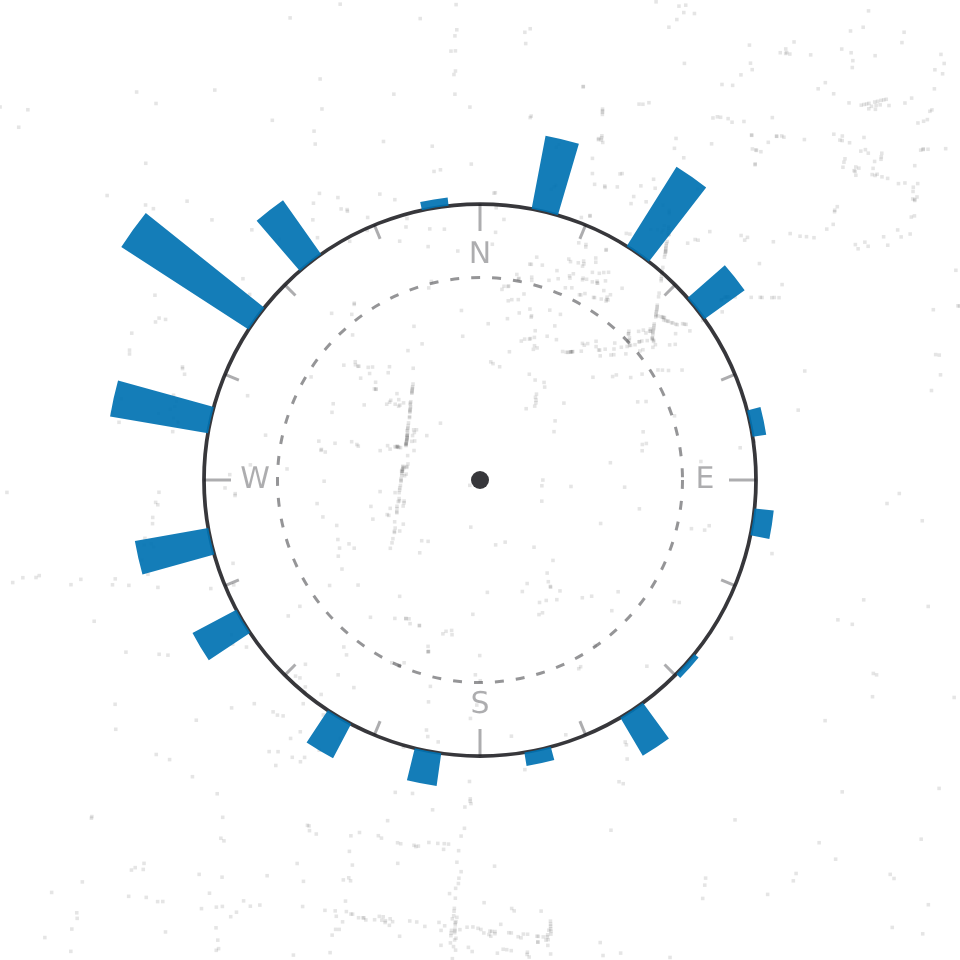
\includegraphics[width=\linewidth]{figures/c-continuum-1}\caption*{\small 1 lens}
  \end{subfigure}\hfill
  \begin{subfigure}[t]{0.24\textwidth}\centering
    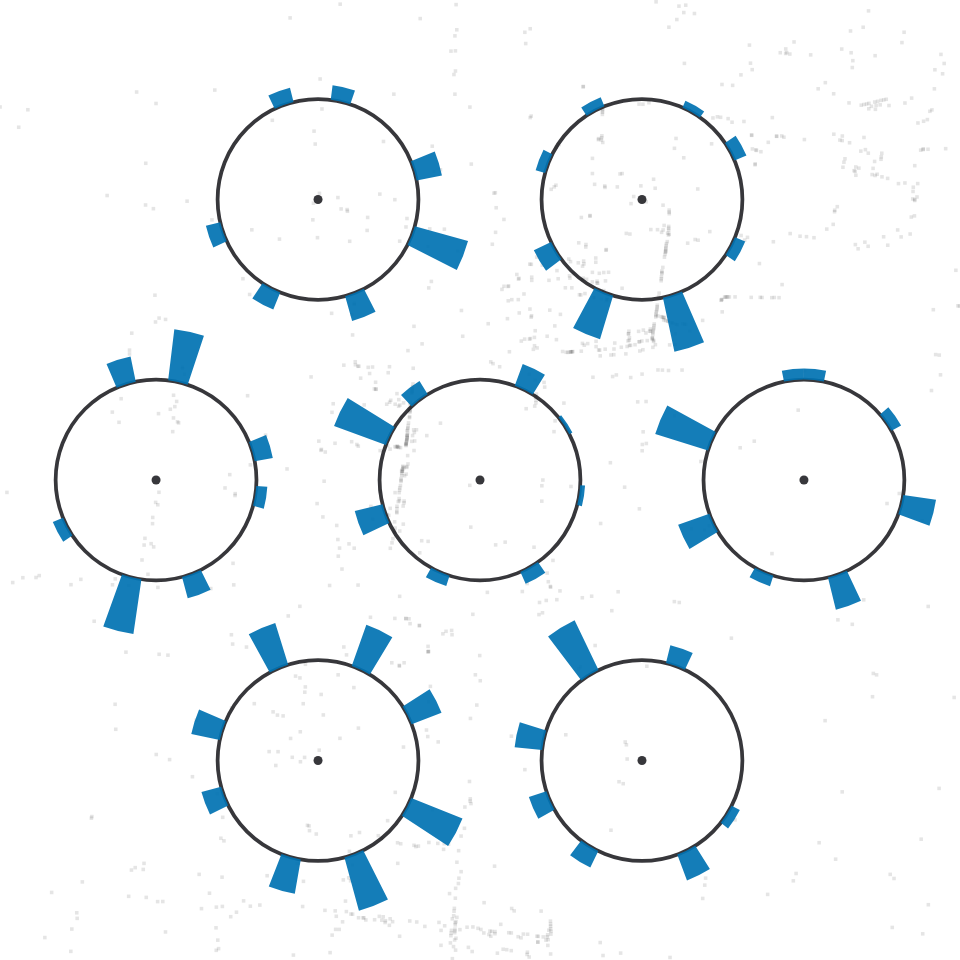
\includegraphics[width=\linewidth]{figures/c-continuum-7}\caption*{\small 7 lenses}
  \end{subfigure}\hfill
  \begin{subfigure}[t]{0.24\textwidth}\centering
    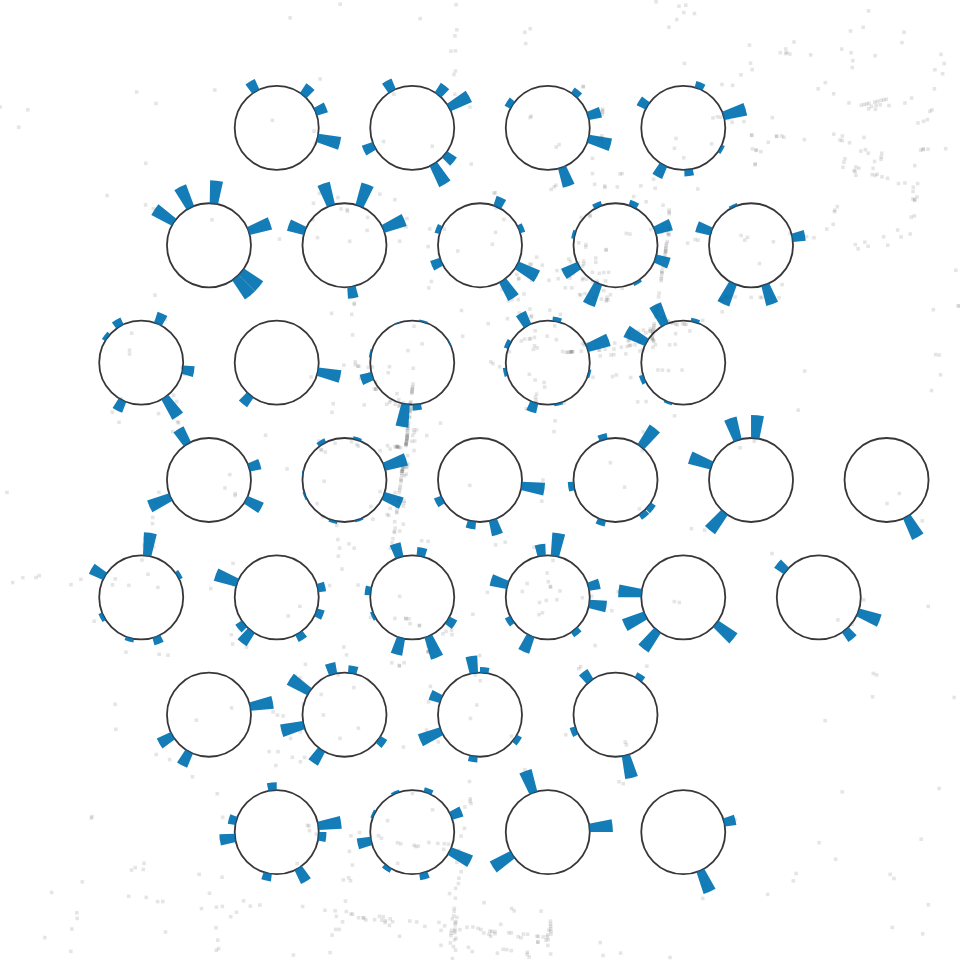
\includegraphics[width=\linewidth]{figures/c-continuum-40}\caption*{\small 37 lenses}
  \end{subfigure}\hfill
  \begin{subfigure}[t]{0.24\textwidth}\centering
    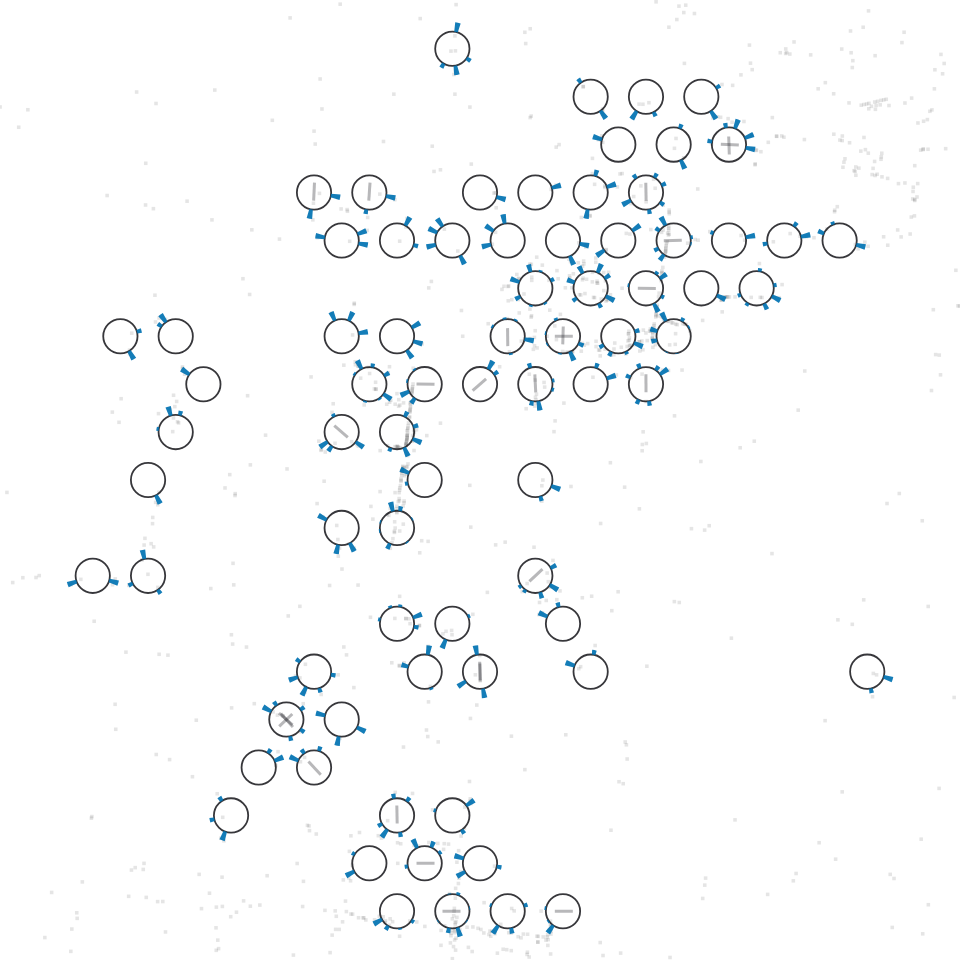
\includegraphics[width=\linewidth]{figures/c-continuum-240}\caption*{\small 241 lenses}
  \end{subfigure}
  \caption{One parameter---the number of lattice centres---takes a single
  bearing-faithful lens to a gridded glyphmap. Every panel is the same binning
  (bearing sectors), the same solver and the same renderer; only the lattice
  changes. Lenses with fewer than three members are not drawn. Grey dots are
  the members.}
  \label{fig:continuum}
\end{figure*}

% ---------------------------------------------------------------------------
\section{Implementation}
\label{sec:implementation}

\sys\ is an open-source JavaScript library (MIT licence)
\todo{repository is private; make it public or deposit an archived snapshot
(e.g.\ Zenodo DOI) before submission, and cite that}. The core is a set of
pure functions over plain objects with no dependency on a map, the DOM or a
framework; it returns geometry, which a canvas renderer paints and a MapLibre
adapter positions on a map. The seven stages of \cref{sec:model} are the API:
a lens is configured by one object per stage, and every figure in this paper is
a single call with different arguments.

\paragraph{The core has no map in it.} The gallery from which
\cref{fig:gallery} is drawn runs the whole pipeline onto bare canvases with no
map library on the page. It doubles as a standing test that the core has not
acquired a rendering dependency. All raster figures in this paper are
regenerated from the library by a script in the repository
(\texttt{paper/scripts/figures.mjs}), which serves the repository, renders the
gallery and a figure page in headless Chromium, and saves each canvas.

\paragraph{Placement.} The necklace solver of \cref{sec:placement} is
independent of the rest of the library and exported on its own. It tries every
cut of the cycle and solves each exactly: by weighted pool-adjacent-violators,
or by its bounded variant when marks have feasible intervals. That makes
order-preserving placement exact, as argued there. An implementation of Speckmann and
Verbeek's algorithms is part of CartoCrow, a C++ framework for cartographic
algorithms from the Applied Geometric Algorithms group at TU
Eindhoven~\cite{cartocrow}. Its project page lists no paper for the framework
itself, so we cite the page. We found no earlier JavaScript implementation. On
2026-09-25 we searched the npm registry for \emph{necklace map},
\emph{necklace maps}, \emph{necklace}, \emph{Speckmann}, \emph{boundary
labeling} and \emph{ring map}. We also ran web and code searches for necklace
maps with JavaScript, d3, npm and GitHub, and a search of Observable. The
only npm package named \texttt{necklace} is an unrelated pipeline library.
This is a search result, not a proof of absence.

\paragraph{Fields.} A field calls the single-lens pipeline once per lattice
centre and changes nothing else. It adds two things a single lens does not
need: a lattice (hexagonal, square, triangular, or a Lloyd-relaxed centroidal
Voronoi tessellation inside a boundary, built on a Delaunay triangulation) and a
uniform grid index so that $m$ lenses over $n$ members do not cost $O(nm)$
distance tests.

Of the evaluation strategies used for toolkit research---demonstration,
usage, technical benchmarks and heuristics~\cite{ledo2018toolkits}---this paper
uses the first and third: the gallery and the coding of
\cref{sec:descriptive,sec:generative} are demonstrations, and
\cref{tab:timing} is a benchmark. A usage study with developers is not part of
this work.

\paragraph{Tests and performance.} The repository has 200 unit tests (Node's
built-in runner, no runtime dependencies), covering among other things
non-overlap, stability and overflow of the solver. \Cref{tab:timing} reports
median wall-clock times for the pure pipeline, without rendering, on the bundled
extract of 1{,}449 OpenStreetMap places.

\begin{table}[t]
  \centering
  \small
  \caption{Median time of the pure pipeline (no rendering), Node~22 on one
  core of a 2.8\,GHz Intel Xeon, 1{,}449 places; produced by
  \texttt{paper/scripts/bench.mjs}. Field sizes are the actual lattice counts.}
  \label{tab:timing}
  \begin{tabular}{@{}lr@{}}
    \toprule
    Configuration & ms \\
    \midrule
    One lens, 8 bearing sectors, necklace placement & 0.9 \\
    One lens, 24 bearing sectors & 1.2 \\
    One lens, 72 bearing sectors & 3.3 \\
    One lens, 8 sectors $\times$ 4 categories, stacked & 0.9 \\
    Field of 37 lenses, 8 sectors each & 5.2 \\
    Field of 241 lenses & 14.1 \\
    Field of 889 lenses & 17.1 \\
    \midrule
    Solver alone, 24 marks, 80\% fill & 0.4 \\
    Solver alone, 72 marks & 1.3 \\
    Solver alone, 288 marks & 17.1 \\
    \bottomrule
  \end{tabular}
\end{table}

The field of 889 lenses is only slightly slower than the field of 241 because 804 of its
lenses (and 165 of the 241) hold fewer than the minimum of three members and are
skipped after the index query, so the cost is dominated by the lenses actually
drawn (85 and 76 respectively). The solver
is $O(K^2)$ in the number of marks, which is immaterial at the bin counts a
lens uses and visible at 288.

% ---------------------------------------------------------------------------
\section{Evaluation plan}
\label{sec:evaluation}

\todo{This section describes a study that has \emph{not} been run. No result
in this draft comes from participants. Replace with the study once it is
pre-registered and run; until then the core claim of \cref{sec:model}---that
bearing-faithful placement helps---is a design conjecture and must be worded as
one everywhere.}

The model's descriptive and generative power is argued in
\cref{sec:descriptive,sec:generative}; its central design claim is empirical and
untested. Two of its axes make testable predictions, and they interact, so we
plan one controlled, within-subjects study crossing them.

\paragraph{Factors.} \emph{Angle}: categorical (block placement, angle
carries category order) versus bearing (necklace placement, angle carries
bearing). \emph{Anchor}: closed ring versus unrolled axis with leaders. A third,
between-trials factor manipulates \emph{displacement}---the gap between a
mark and its true bearing, at four levels from 0 to 45\,degrees
\todo{levels to be fixed by pilot}---to locate the point at which a displaced
mark misleads (the open policy question of \cref{sec:association}).

\paragraph{Tasks.} Five tasks, each with a ground truth computable from the
stimulus:
\begin{enumerate}[leftmargin=*, itemsep=1pt]
  \item \textbf{Direction}: ``In which direction from the centre is category
    $X$ most concentrated?'' Response: a bearing; error in degrees.
  \item \textbf{Isotropy}: ``Is $X$ spread evenly around the centre?''
    Ground truth from the resultant length $R$.
  \item \textbf{Comparison}: ``Which of two highlighted directions has more
    $X$?'' Accuracy.
  \item \textbf{Composition}: ``Which category is most common inside the
    lens?'' Accuracy. The categorical ring should do at least as well here;
    the task is included so that a win on direction is not bought silently.
  \item \textbf{Association}: ``Click the part of the map that the highlighted
    mark summarises.'' Distance error.
\end{enumerate}

\paragraph{Hypotheses.}
H1: bearing-faithful placement reduces direction error (task~1) relative to
categorical placement.
H2: categorical placement is no worse than bearing placement for composition
(task~4).
H3: the unrolled axis improves comparison accuracy (task~3) relative to the
ring.
H4: the ring beats the unrolled axis on association (task~5) without leaders,
and leaders close the gap.
H5: direction error grows with displacement, and leaders flatten that growth.

\paragraph{Stimuli, participants, analysis.} Synthetic point patterns with
controlled anisotropy (so ground truth is exact) plus a held-out set from real
OpenStreetMap extracts, rendered by the library. Participants recruited online
\todo{platform, $N$ from a power analysis on pilot data, compensation, ethics
approval}. Mixed-effects models with participant and stimulus as random
effects \todo{specify before data collection; pre-register (e.g.\ OSF)}.

\paragraph{Known risk.} A study of off-screen indicators reports that
participants located off-screen objects better, and overwhelmingly preferred,
orthographic rather than radial projection onto the viewport border
\cite{jackle2017topology}. That is evidence \emph{against} direction-preserving
placement on a boundary, in a closely related setting; our hypotheses H1 and
H5 should be read as the direct test of whether it transfers to a lens.
\doubt{Exact result, $N$ and task of Jäckle et al.\ to be confirmed from the
full text before this paragraph is kept.}
Relatedly, a study of orbital boundary labels around a circle reports straight
leaders faster than orbital-radial ones at similar accuracy
\cite{wallinger2026clarity}; our leaders are straight.
\doubt{Pending the citation audit.}

% ---------------------------------------------------------------------------
\section{Discussion and limitations}
\label{sec:discussion}

\paragraph{A mean bearing is not always a direction.} Positioning a
category's mark at the circular mean of its members is only honest when they
are concentrated. On the demonstration data all four categories' means fell
within about twenty degrees of each other, because the whole dataset is denser
to the north-west \todo{re-measure and report the actual spread from the
bundled data rather than the development log}: the bearing-faithful ring
collapsed into a bundle and lost the composition reading the categorical ring
gave for free. The morph from category order to bearing is therefore strongest
for spatially segregated categories. Two responses are built: marks are faded
by their resultant length $R$, and the \emph{cross} binning (bearing
$\times$ category) gives each category one mark per sector, so that a diffuse
category shows as a spread of marks rather than one misplaced one. We regard
the second as the honest multivariate view and the first as a limitation to be
stated, not a fix.

\paragraph{How multivariate is this?} Most configurations in this paper
summarise one categorical variable by count. Several variables are supported
through cross binning, stacked necklaces (one per variable, exact angular
fidelity at the cost of radial space), and areal measures with declared
extensive or intensive semantics; but we have not shown that these scale beyond
a handful of variables, and the glyph literature suggests they will not
without careful design~\cite{borgo2013glyph,fuchs2017glyph}.
\todo{Either demonstrate a genuinely multivariate census case (e.g.\ several
deprivation domains) or narrow the claim in the title and abstract.}

\paragraph{Relation to geographically weighted statistics.} A field of
disc-shaped lenses on a lattice computes, at each centre, local summaries with
a uniform (hard cut-off) kernel---which is geographically weighted summary
statistics with the simplest kernel~\cite{brunsdon2002gwss}, and a field drawn
as glyphs is close to a tilemap of such summaries~\cite{slingsby2018tilemaps}.
We do not claim the statistics. What the lens adds is (i) keeping the
within-lens decomposition by bearing and distance, drawn at its true bearing,
where a GW summary is one scalar per location, and (ii) one model in which the
single lens and the field are the same object at different settings.
\todo{Implement bi-square and Gaussian kernels so that the field reproduces GW
summary statistics exactly, and show it; this turns the obvious reviewer
objection into a validity check.}
\doubt{Readings of Brunsdon et al.\ (kernel choice) and of Slingsby's tilemaps
are pending the citation audit.}

\paragraph{The continuum has a usable range.} As the lattice densifies each
ring shrinks, and below roughly ten pixels of ring radius a glyph stops
carrying multivariate information and the field reads as a density surface with
texture \doubt{an observation from building the demonstrations, not a measured
threshold}. This is the trade between spatial and multivariate resolution that
any glyph map makes; the renderer sheds labels and compass as rings shrink, but
the threshold itself is a candidate for the study.

\paragraph{Lenses do not tessellate.} Centres on a lattice tessellate the
plane; the discs they select do not. At touching packing (disc radius half the
nearest-neighbour spacing) a hexagonal lattice covers
$\pi/(2\sqrt3)\approx90.7\%$ of the ground, a square lattice
$\pi/4\approx78.5\%$ and a triangular (honeycomb) lattice
$\pi/(3\sqrt3)\approx60.5\%$. Any larger disc makes neighbours overlap and
count some members twice, while on a hexagonal lattice the gaps do not close
until the disc radius reaches the cell's circumradius, $s/\sqrt3$: between
$s/2$ and $s/\sqrt3$ a field both misses ground and double-counts it, so no
disc radius is both gap-free and overlap-free. Drawing only the cell would be
the comfortable lie, so the field reports coverage and can draw the disc, the
cell, or both.

\paragraph{Other limitations.} Bearing from a polygon's centroid is ambiguous
for elongated or concave units, where the population-weighted centroid, the
geometric centroid and the unit's full angular extent disagree. The baseline
for the location quotient (complement, region, nation) changes the reading and
should be visible, not a configuration default. Placement is exact only in the
common case (\cref{sec:placement}). Web Mercator distorts area, so densities are
computed geodesically rather than from screen space.

\paragraph{Name.} The library's working name collides with an unrelated
occlusion-management technique for 3D glyph fields~\cite{tong2017glyphlens};
it will be renamed before publication.

\section{Conclusion}
\label{sec:conclusion}

A lens that summarises the data under it has to answer two questions that a
magnifying lens does not: what to summarise, and where to put the summary. We
split Tominski et al.'s lens function and join into three stages each, and
showed that in the resulting seven-stage space a category ring, a
bearing-faithful necklace, a route profile and a gridded glyphmap are points
reached by changing arguments rather than by writing new techniques. The part
of the space we find most interesting is where the lens boundary itself carries
data: a ring whose angle means bearing, whose marks are tied back to the ground
by leaders when placement or unrolling gives adjacency away, and whose radius
control shows how fragile the reading is. Whether that helps anyone is the
question the planned study exists to answer.


\bibliographystyle{plainnat}
\bibliography{references}

\appendix
\onecolumn
% ---------------------------------------------------------------------------
% Citation audit. For co-authors; remove before submission.
\section*{Appendix: citation audit (remove before submission)}
\label{sec:audit}

Every entry in the bibliography was checked on 2026-09-23 and 2026-09-25 against its registry
record---Crossref, or DataCite for the Eurographics (10.2312), Dagstuhl
(10.4230) and arXiv (10.48550) DOIs---or, where there is no DOI, against the
page at its URL. The table records, for each source, the evidence behind what
this draft says about it: \textbf{F} read in full (``pre'' marks a preprint or
author copy rather than the version of record), \textbf{A} abstract only,
\textbf{M} bibliographic record only, \textbf{W} web pages. Verbatim quotes with
page references are in \texttt{paper/citation-audit.md}.
\texttt{paper/scripts/check-bib.mjs -{}-online} repeats the registry check; on 2026-09-25 all 67 DOIs resolved and every registered title matched.

\begingroup
\small
\setlength{\LTcapwidth}{\textwidth}
\renewcommand{\arraystretch}{1.1}
\begin{longtable}{@{}p{3.2cm}p{1.0cm}p{5.6cm}p{6.6cm}@{}}
\toprule
Source & Ev. & Used for & Caveat \\
\midrule
\endhead
\bottomrule
\endfoot
\multicolumn{4}{@{}l}{\emph{Lens models and design-space method}}\\
\src{bier1993toolglass} & F & origin of magic lenses & --- \\
\src{bier1994taxonomy} & F & taxonomy of see-through tools & a taxonomy of see-through tools in general, not of lenses; several same-title DOIs exist \\
\src{fox1998composing} & F & composing lenses & a programming-model contribution (delegation), not a visual one \\
\src{tominski2014star} & F & $\Sel$/$\Jn$ model; data types and tasks; future directions (combination, toolkit) & the symbol $\lambda$ is not in the 2014 STAR; neither survey lists adaptive lenses or evaluation as future directions \\
\src{tominski2017survey} & F pre & $\lambda$ notation; effect extent (interior, side effects, separate view) & online 2016, issue 2017 \\
\src{mota2025design} & F & seven dimensions; effect scope and encoding values; 45-paper corpus & arXiv v2 only; no published version found \\
\src{dai2026mapping} & A & five-phase construction process & full text not accessed; nothing about how it evaluates design spaces is used \\
\src{beaudouinlafon2004designing} & F & descriptive, evaluative, generative power & --- \\
\src{ledo2018toolkits} & F & toolkit evaluation strategies & --- \\
\multicolumn{4}{@{}l}{\emph{Lenses and probes on maps}}\\
\src{tong2017glyphlens} & A & name collision; occlusion lens for 3D glyphs & --- \\
\src{hurter2011moleview} & F & semantic lens that pushes elements to its border & author order is Hurter, Ersoy, Telea (several surveys have it wrong) \\
\src{pindat2012jellylens} & F & content-adaptive lens shape & --- \\
\src{zhang2020clusterlens} & F & re-aggregation inside a lens & no charts or ring \\
\src{karnick2010route} & F pre & detail lenses on the map border in route order; leaders to first and last only; direction-coherence cost & preprint \\
\src{ellis2005sampling} & F & sampling lens; aggregates as future work & scatterplots and parallel coordinates, not maps \\
\src{dumas2015vectorlens} & F & ring encoding direction for selection & online 2014, issue 2015; no map example \\
\src{butkiewicz2008probes} & F & probes: region + user-placed pane of charts, linked by line or colour & --- \\
\src{butkiewicz2010maup} & F pre & MAUP alerts between compared regions; scale component explicitly excluded & read the anonymised EuroVis submission, not the published version \\
\src{kruger2013trajectorylenses} & A & set-operation lenses; aggregates near the lens or in colour-matched panels & full text not accessed (open copy withdrawn); verbatim related-work excerpts only \\
\src{scheepens2016traffic} & A & selection widget by area and direction; annotation windows & whether it is called a lens, and where windows sit, unverified \\
\src{ma2020gtmaplens} & A & movable lenses over geo-text & what is shown and where, unverified \\
\src{tominski2012stacking} & F pre & time lens: ring of cyclic time bins around a query circle & ring placement around the circle strongly implied, not stated \\
\src{visquill} & W & shipped aggregating ring lens on maps & angle meaning not documented; Lab blueprint spaces one bar per category \\
\multicolumn{4}{@{}l}{\emph{Labelling around a focus region}}\\
\src{fekete1999excentric} & F pre & left/right label stacks; radial variant orders by bearing; summary glyph as future work & read the HCIL tech report; its study numbers differ from how others report them---do not quote them \\
\src{bertini2009extended} & A & density extensions; ``summary statistics'' & what the statistics are is unverified \\
\src{fink2012focus} & F pre & labels on the circle; radial ports; conflicts dropped; clustering variant; focus placement & --- \\
\src{haunert2014labeling} & A & leaders to the centre; one position per label; real-time JavaScript & --- \\
\src{heinsohn2014boundary} & A & moving focus regions & mechanism for coherence unverified; biological networks \\
\src{niedermann2019focus} & A & fisheye displacement; optimisation when the focus stops & program type unverified \\
\src{bekos2019external} & F pre & external-labelling taxonomy & arXiv v2 \\
\src{bonerath2024orbital} & F & orbital arc labels; minimum leader length & --- \\
\src{wallinger2026clarity} & F pre & $n=54$; straight leaders faster, similar accuracy & numbers from arXiv v1, not the PacificVis version \\
\src{gedicke2021zoomless} & F pre & labels along the map's lower edge & vol.\ 27 (2021) despite a 2020 DOI \\
\multicolumn{4}{@{}l}{\emph{Glyph maps and within-cell structure}}\\
\src{ward2002taxonomy} & F pre & data-driven vs structure-driven placement & author manuscript \\
\src{borgo2013glyph} & F & glyph design guidance & DataCite lists 2012 in error; pages from the DOI suffix \\
\src{fuchs2017glyph} & F pre & 64 studies; layout and map backgrounds understudied & --- \\
\src{wickham2012glyphmaps} & F pre, A & glyphs at the data's own grid locations & quote the version of record's abstract where possible \\
\src{mcnabb2019multivariate} & A, F pre & hierarchical-centroid placement with LOD & --- \\
\src{slingsby2018tilemaps} & F & tilemaps; GW outputs \emph{proposed}; grid resizing and larger kernels discussed & workshop paper, no DOI; GW use not demonstrated \\
\src{slingsby2023gridded} & F pre & screen-space grid re-aggregated on zoom; within-cell heterogeneity as future work & --- \\
\src{laksono2024gridded} & F & gridded glyphmaps for GMCDA & no user study \\
\src{trautner2022honeycomb} & F pre & diamond cut; $n=42$ study; the C3 sentence & the quoted sentence concerns colour-only hexbins; amber inclusions untested \\
\src{kawakami2024hextiles} & F & variance-based per-tile confidence & arXiv only; no formula; study ($n=7$) without the variance encoding, no significant effects \\
\src{boeing2019urban} & F pre & polar histograms of street bearings & bearing of edges, not from a centre \\
\src{gleicher2011comparison} & A & juxtaposition, superposition, explicit encoding & --- \\
\multicolumn{4}{@{}l}{\emph{Local statistics, scale and point patterns}}\\
\src{brunsdon1996gwr} & A & origin of GW methods & the ``sudden cut-off'' reading is unverified and not used \\
\src{brunsdon2002gwss} & A & GW summary statistics & whether it names a uniform kernel is unverified \\
\src{dykes2007gwvis} & F pre & ``moving spatial window mean smoother''; scalograms; regular grid; directed weighting & Gaussian kernel; $h$ precomputed, not a slider; check the sign in the directed-kernel formula before reproducing it \\
\src{goodwin2016multiple} & F pre & local correlation across scale & --- \\
\src{anselin1995lisa} & A & local indicators & --- \\
\src{openshaw1984maup} & F (scan) & MAUP: scale and aggregation problems & reviews and defines the problem, does not introduce it; year not printed in the scan \\
\src{fotheringham1991maup} & A & MAUP unpredictable in multivariate analysis & --- \\
\src{ripley1977modelling} & F & $K(t)=\pi t^2$ under Poisson; envelopes & the $L$-function is not in the paper body \\
\src{getis1987second} & A & point-centred second-order analysis & the $L_i$ formula is unverified and not used \\
\src{wiegand2004rings} & A & circle vs ring statistics; null models & ``envelopes'' not verified in this paper \\
\src{yamu2016fractal} & F & radial (mass--radius) analysis & a planning-theory paper; a methods citation would be better \\
\src{willett2007scented} & F & scented widgets & credits histogram sliders to earlier work \\
\src{mardia1999directional} & M & circular mean, resultant length, circular SD & book not accessed; definitions are standard but the equation numbers are unverified \\
\multicolumn{4}{@{}l}{\emph{Off-screen indicators, necklace maps, ring maps}}\\
\src{speckmann2010necklace} & F pre & regions projected onto intervals; symbols without overlap; multiple necklaces; max scale then centring; ``do not need leaders'' & --- \\
\src{speckmann2015algorithms} & F pre & fixed order $O(n\log n)$; any order NP-hard (wedge intervals); bearing order not always optimal for max scale & accepted manuscript; objective differs from ours \\
\src{stewart2011ringmaps} & F & evenly spaced spokes, one per unit; a leader for every spoke & ordering rule of spokes not verified \\
\src{tominski2016comparing} & F pre & ring slots with arcs toward originals; direction-ordered slots only suggested & --- \\
\src{jackle2017topology} & F pre & $n=18$; 94.4\% orthographic; radial familiar with a point of interest & arXiv v1 only; rectangular border \\
\src{baudisch2003halo} & M & off-screen proxy (via Jäckle et al.'s classification) & own text not read \\
\src{zellweger2003citylights} & M & off-screen proxy (via Jäckle et al.) & own text not read \\
\src{gustafson2007edgeradar} & M & border region (via Jäckle et al.) & own text not read \\
\src{gustafson2008wedge} & M & off-screen proxy (via Jäckle et al.) & own text not read \\
\src{jackle2015ambient} & M & aggregated border grid (via Jäckle et al.) & own text not read \\
\src{danyluk2026ringmaps} & A (partial) & AR ring maps for pedestrian navigation & how landmarks are placed is unverified \\
\src{draper2009radial} & M & survey of radial methods (its title) & --- \\
\end{longtable}
\endgroup


\end{document}
